\chapter{Multiparty Cardinality Testing}


\section{Neues am Paper}
Diese Arbeit basiert auf dem Protokoll, das in \cite{Doettling2021} vorgestellt wurde. Es gab schon vorher einige Veröffentlichungen zum Thema Private Set Intersections, auf denen das Paper aufbauen kann. Zuerst wurden Protokolle für zwei Parteien entworfen, dann auch für mehrere Parteien. Das Paper
\cite{Ghosh2019} ist die letzte Veröffentlichung, auf der das Protokoll aufbaut.\\
Die große Neuerung in der Veröffentlichung \cite{Ghosh2019} ist, dass die Kommunikations-Komplexität nun vor allem von O(t) und nur noch logarithmisch von O(n) abhängt. \cite{Ghosh2019}\\
Das von Gosh vorgeschlagene Cardinality Testing ist jedoch noch nicht  für mehrere Parteien optimiert. Daher ist das neue Protokoll zur Bestimmung der Schnittmengen-Größe die wichtigste Neuerung des Papers \cite{Doettling2021}


\section{Abwandlungen zum Paper}
Das Protokoll wurde offensichtlich entworfen um auch mit mehreren teilnehmenden Parteien effizient zu sein.
Das Paper \cite{Doettling2021} nutzt also in vielen Unterprotokollen Broadcast-Funktionen.

Beispiel: secRank \cite{Doettling2021}
\begin{lstlisting}[firstnumber=1]
Each party Pi broadcasts an encrypted uniformly chosen at
random unit upper and lower triangular Toeplitz matrices...
\end{lstlisting}

Beispiel: secMult \cite{Doettling2021}
\begin{lstlisting}[firstnumber=6]
Each party Pi computes [...] and broadcasts c(i).
\end{lstlisting}

Ich habe versucht, nah an die Spezifizierungen des Papers ran zu kommen, doch 
um die Implementierung des Protokolls zu vereinfachen und um das Testen der Implementierung zu erleichtern, habe ich das System etwas abgewandelt. In meiner Implementierung gibt es einen Koordinator. Dieser Koordinator erleichtert das testen enorm, denn durch ihn kann sicher gestellt werden, dass alle "verschickten" Informationen immer zum richtigen Zeitpunkt am richtigen Ziel ankommen.\\
Diese Änderung wird die Sicherheit des Protokolls nicht schwächen, weil alle Informationen, per Broadcast verschickt werden immer verschlüsselt sind.
Auch wenn Daten entschlüsselt werden, sind sie immer für einen Angreifer, der Informationen über die Eingabemengen erhalten will nutzlos. Ein gutes Beispiel dafür ist das Unterprotokoll secInv \\

\begin{figure}[h]
\begin{center}
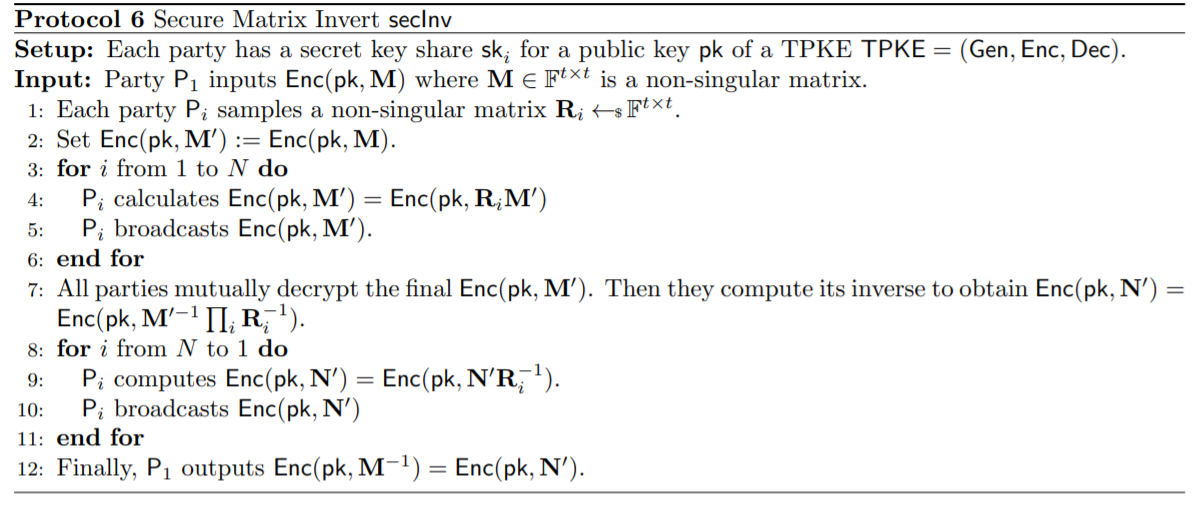
\includegraphics[width = 15cm]{secInv.png}
\caption{Teil-Protokoll secInv}
\cite{Doettling2021}
\label{oInv}
\end{center}

\end{figure}

Hier wird zwar eine Matrix entschlüsselt (7), diese ist aber randomisiert(1-5), also nutzlos, außer, man besitzt eine der geheimen Matrizen(9), die ja nicht verschickt werden.\\
Das Protokoll ist also auf eine Art und Weise aufgebaut, dass kein passiver Zuhörer irgendwelche nützlichen Informationen aus den Nachrichten, die zwischen den Parteien verschickt werden, gewinnen kann. Also kann auch ein Angreifer, der alle Nachrichten zwischen den Teilnehmern des Protokolls keine Informationen extrahieren. Also können wir auch sicher sein, dass, selbst wenn der Koordinator von einem Angreifer kontrolliert wird, die verschlüsselten Eingabedaten sicher sind.\\
Die neue Struktur, die einfacher zu implementieren und testen ist, macht das Protokoll also nicht weniger sicher. Besonders deshalb, weil das Protokoll so konstruiert ist, dass selbst alle verschickten Nachrichten zusammen keine geheimen Daten preisgeben.\\

Die meisten der Unterprotokolle bestehen aus sich abwechselnden Teilen von Kommunikation zwischen den Parteien und Berechnungen der Parteien. Also habe ich die Unterprotokolle implementiert, indem die Berechnungen der Parteien in Abschnitte aufgeteilt sind, die dann von dem Koordinator aufgerufen werden können. Gut zu sehen ist das beispielsweise im Teil-Protokoll MPCT, wo der Koordinator nur die Koordinierung der Parteien übernimmt, indem die Parteien die richtigen Eingaben zum richtigen Zeitpunkt bekommen.\\

\begin{lstlisting}
public boolean MPCT(List<BigInteger> inputAlphas, BigInteger setMod){
        MPCTCounter++;

        List<List<EncryptedNumber>> encPointsList = new LinkedList<>();
        //line 1 already done in setup

        //line 2
        for (int i = 0; i < parties.size(); i++) {
            encPointsList.add(parties.get(i).MPCTpart1(inputAlphas, setMod));
        }
        //line 3
        return parties.get(0).MPCTpart2(encPointsList, inputAlphas, t);
    }


\end{lstlisting}

Das ist die einfachste Möglichkeit, um zu erreichen, dass alle Parteien zum richtigen Zeitpunkt das richtige Berechnen, denn einige der Berechnungen hängen auch von den gesendeten Nachrichten der anderen Parteien ab.\\


\section{andere Veröffentlichungen}
Es gibt einige andere Veröffentlichungen in den letzten Jahren, die sich mit ähnlichen Problemen oder sogar dem gleichen Problem beschäftigen.
Das Problem der Private Threshold Set Intersection lässt sich in zwei Teilprobleme aufteilen. Zum Einen in das Berechnen der Schnittmenge, worauf Gosh sich in \cite{Ghosh2019} konzentriert, und das sogar noch erweitert wurde, um auch für mehr als 2 Parteien nutzbar zu sein.\cite{Doettling2021}  Und zum anderen in der Ermittlung der Größe der Schnittmenge. Das ist der Fokus des Papers \cite{Doettling2021}. Aber auch Badrinarayanan \cite{cryptoeprint:2020:600} beschäftigt sich mit der Ermittlung der Größe der Schnittmenge. Badrinarayanan nutzt jedoch andere kryptographische Annahmen und erhält die Ergebnisse mithilfe von anderen mathematischen Grundlagen. \cite{Doettling2021}\\
Es gibt also viele neue Entwicklungen in diesem Bereich, die für unterschiedliche Zwecke genutzt, oder kombiniert werden können, um die besten Ergebnisse zu erreichen. Das Protokoll aus \cite{Doettling2021} ist also eine relevante Neuerung und eine Analyse kann helfen, die Effizienz dieser Neuerung mit anderen zu vergleichen.

